\documentclass[11pt,pdftex,letter]{article}
%\documentclass[11pt]{llncs}
%\documentclass[11pt,pdftex]{article}
%\documentclass{sig-alternate-10pt}
%\usepackage{amsthm}
%\usepackage{algorithm}
%\usepackage[noend]{algorithmic}
\usepackage[lined,boxed,commentsnumbered]{algorithm2e}

%[[For jpeg images]]
%\usepackage{pgf}

\usepackage{amssymb}
\usepackage{comment}
\usepackage{amsmath}
%\usepackage{graphicx}
%\usepackage{color}
\usepackage{fullpage}
%\usepackage[pdftex]{graphicx}
%\DeclareGraphicsRule{*}{mps}{*}{<++>}

\ifx\pdftexversion\undefined
\usepackage[dvips]{graphicx}
\else
  \usepackage[pdftex]{graphicx}
  \DeclareGraphicsRule{*}{mps}{*}{}
\fi


\def\lf{\tiny}
\def\rrnnll{\setcounter{linenumber}{0}}
\def\nnll{\refstepcounter{linenumber}\lf\thelinenumber}
\newcounter{linenumber}

\usepackage[usenames,dvipsnames]{color}
%\usepackage[caption=true,font=footnotesize]{subfig}
\usepackage{subfigure}
%\usepackage{xspace} 	% Guesses whether a space is needed when invoked
\usepackage{listings}
\usepackage{url}
\usepackage{wrapfig}
\usepackage{cite}
%\usepackage{framed}
\usepackage{framed,color}
\definecolor{shadecolor}{rgb}{0.9,0.9,0.9}
%
\usepackage[boxed]{algorithm2e}
%\usepackage{comment}

%[[PKto change spacing
%\usepackage{titlesec}
%\titlespacing\section{0pt}{7pt}{6pt}
%]]

%\newtheorem{theorem}{Theorem}[section]
%\newtheorem{takeaway}[theorem]{Takeaway}
%\newtheorem{fact}[theorem]{Fact}


%\pdfpagewidth=8.5in
%\pdfpageheight=11in

% url.sty was written by Donald Arseneau. It provides better support for
% handling and breaking URLs. url.sty is already installed on most LaTeX
% systems. The latest version can be obtained at:
% http://www.ctan.org/tex-archive/macros/latex/contrib/misc/
% Read the url.sty source comments for usage information. Basically,
% \url{my_url_here}.

\newcommand{\CPO}{\textsc{FixTag}}
\newcommand{\DPO}{\textsc{ReuseTag}}
\newcommand{\PS}{\textsc{PS}}
\newcommand{\Bit}{\textsc{Bit}}

\newcommand{\gns}{Global Network State\xspace}
\newcommand{\GNS}{\textsc{GNS}\xspace}

%\newtheorem{theorem}{Theorem}[section]
%\newtheorem{lemma}{Lemma}[section]
%\newtheorem{claim}{Claim}[section]
%\newtheorem{scenarios}{Scenarios}[section]
%\newtheorem{observation}{Observation}
%\newtheorem{takeaway}{Takeaway}[section]
%\newtheorem{definition}{Definition}


%
%
% carry over Herald's group cool way of marking changes
\definecolor{heraldBlue}{rgb}{0.0,0.0,0.8}
\definecolor{heraldRed}{rgb}{0.8,0.0,0.0}
\definecolor{heraldGray}{rgb}{0.4,0.4,0.4}
\definecolor{heraldBlack}{rgb}{0.0,0.0,0.0} %removes comment color
\definecolor{heraldGreen}{rgb}{0.0,0.4,0.0} %removes comment color
\def\r#1{\textcolor{heraldBlue}{\em #1}}
\def\q#1{\textcolor{heraldRed}{\em #1}}
\def\d#1{\textcolor{heraldBlue}{#1}}
\def\R#1{\textcolor{heraldBlue}{#1}}
\def\D#1{\textcolor{heraldBlue}{#1}}
%
%\DeclareMathOperator{\respc}{res}

\newcommand{\len}{\text{d}}

\newcommand{\nodes}{\mathcal{N}}
\newcommand{\links}{\mathcal{E}}
\newcommand{\epoints}{\Pi}
\newcommand{\epoint}{\pi}
\newcommand{\legsw}{\mathcal{L}}
\newcommand{\sdnsw}{\mathcal{S}}
\newcommand{\sw}{\legsw\sqcup\sdnsw}
\newcommand{\fset}{FS}

\newcommand{\Cost}{\gamma}

\newcommand{\ft}{ft}

\newcommand{\eepath}{p}
\newcommand{\link}{e}

\newcommand{\dom}{\textit{dom}}
\newcommand{\pr}{\textit{pr}}
\newcommand{\CPOs}{\textit{paths}}
\newcommand{\seq}{\textit{seq}}
\newcommand{\cur}{\textit{cur}}
\newcommand{\Tag}{\textit{tag}}


\newcommand{\ports}{\Pi}
\newcommand{\seport}{\pi}
\newcommand{\inports}{\overrightarrow{\ports}}
\newcommand{\swports}{\overleftrightarrow{\ports}}
\newcommand{\seinports}{\epoints^{\bullet}}
\newcommand{\seinportsone}{\seinports_1}
\newcommand{\seinportstwo}{\seinports_2}
\newcommand{\seinportsthree}{\seinports_3}
\newcommand{\neinports}{\epoints^{\circ}}

\newcommand{\readt}{\texttt{r}}
\newcommand{\writet}{\texttt{w}}
\newcommand{\op}{\texttt{op}}


\newcommand{\cellblocks}{CB}
\newcommand{\cellblock}{c}
\newcommand{\frontier}{\mathcal{F}}
\newcommand{\MIP}{\textsc{Opt}}
\newcommand{\smartparagraph}[1]{\noindent{\bf #1}\ }
\newcommand{\eg}{{\it e.g.}}
\newcommand{\ie}{{\it i.e.}}
\newcommand{\etc}{{\it etc.}}
\newcommand{\etal}{{\it et al.}\xspace}
\newcommand{\id}{{\it id}}

\def\TR{0}
\def\NOTES{1}
\def\SAVESPACE{1}
\def\SHOWAUTHORS{1}
\def\SHOWGIT{0}
% variables may contain the above definitions to control build options at compile-time
%\input{variables}

\if \SAVESPACE 1
%\usepackage{setspace}
%\usepackage{titlesec}
%\titlespacing\section{0pt}{7pt}{6pt}
\usepackage{titlesec}
\titlespacing\section{0pt}{7pt}{6pt}

\fi

\if \NOTES 1
\newcommand{\mcnote}[1]{\textcolor{heraldBlue}{\small \bf [MC: #1]}}
\newcommand{\dlnote}[1]{\textcolor{heraldBlue}{\small \bf [DL: #1]}}
\newcommand{\ssnote}[1]{\textcolor{heraldBlue}{\small \bf [SS: #1]}}
\newcommand{\pknote}[1]{\textcolor{heraldBlue}{\small \bf [PK: #1]}}
%\newcommand{\problem}[1]{\textcolor{heraldRed}{\small \bf [PROBLEM: #1]}}
\else
\newcommand{\mcnote}[1]{}
\newcommand{\dlnote}[1]{}
\newcommand{\ssnote}[1]{}
\newcommand{\pknote}[1]{}
\newcommand{\problem}[1]{}
\fi

%Petr's definitions
\newcommand{\ack}{\textit{ack}}
\newcommand{\nack}{\textit{nack}}
\newcommand{\rmw}{\textit{rmw}}
\newcommand{\State}{\mathit{States}}
\newcommand{\ignore}[1]{}
\newcommand{\Pb}{CPC}
\newcommand{\E}{\mathcal E}
%

%[[PK environments for article style
\newtheorem{theorem}{Theorem}
\newtheorem{conjecture}[theorem]{Conjecture}
\newtheorem{corollary}[theorem]{Corollary}
\newtheorem{definition}[theorem]{Definition}
\newtheorem{lemma}[theorem]{Lemma}
\newtheorem{observation}[theorem]{Observation}
\newenvironment{proof}[1][Proof]{\noindent\textbf{#1.} }{\hfill $\Box$\\[2mm]}
\newenvironment{proofsketch}[1][Proof sketch]{\noindent\textbf{#1.} }{\hfill $\Box$\\[2mm]}
%]]

\begin{document}
\sloppy

%\title{Distributed Network Programming}
%\title{The Distributed SDN Update Problem:\\Towards Software Transactional Networks}

%\title{On Consistent Updates in Software Defined Networks under Unreliable Control}
%\title{The Case for Reliable Software Transactional Networking}

%\title{A Distributed SDN Control Plane for Concurrent Policy Updates}

\title{Distributed Software-Defined Networking:\\ The ACM PODC 2014 Workshop \textbf{DSDN}}



\author{
Petr Kuznetsov$^{1}$ \quad Stefan Schmid$^{2}$\\
\\
       $^{1}$ T\'el\'ecom ParisTech\\
%, 46 Rue Barrault, 75013 Paris, France\\
        petr.kuznetsov@telecom-paristech.fr\\
\\
        $^{2}$ TU Berlin \& T-Labs \\ %Ernst-Reuter Platz 7, 10587 Berlin, Germany\\
	    stefan.schmid@tu-berlin.de}
%	}

%\institute{}

\date{}


\maketitle


\thispagestyle{empty}

%\if \SAVESPACE 1
%\setlength{\floatsep}{3pt}
%\setlength{\textfloatsep}{3pt}
%\setlength{\dbltextfloatsep}{3pt}
%\setlength{\intextsep}{3pt}
%\setlength{\abovecaptionskip}{3pt}
%\fi

% A category with the (minimum) three required fields
%\category{C.2.1}{Network Architecture and Design}{Centralized Networks}
%\category{C.2.4}{Distributed Systems}{Network Operating Systems}
%\terms{Measurement, Performance}
%\keywords{}



\begin{abstract}
The workshop on Distributed Software-Defined Networking, DSDN, took
place in Paris, France, on the 15th of July, just before
the 33rd ACM Symposium on Principles of Distributed Computing.
The workshop intended to be a forum to discuss new algorithmic and
distributed computing challenges offered by the emerging field of
Software-Defined Networking (SDN).
The workshop consisted of invited and peer-reviewed presentations, both
from researchers in the field of
distributed computing and in the field of networking.
\end{abstract}


\section{SDN: Networking Is Cool Again!}

Computer networking currently goes through a transition phase,
and the paradigm of Software-Defined Networking (SDN)
is discussed intensively, both in the industry and in the academia. In
a nutshell, the paradigm out-sources and consolidates the control over a network
to a logically centralized \emph{software control plane}.
This separation, and the introduction of ``programmability'',
allows to adapt and innovate the network control plane in a more
efficient way and independently of the data plane.
The resulting flexibilities open interesting new opportunities:
networking is considered cool again.

\section{SDN meets PODC}

At the heart of SDN lies the idea to design and operate
the network control logic
on a centralized network view.
However, inevitably, this view is only \emph{logically centralized}~\cite{onix}:
in order to avoid a single point of failure and ensure scalability and efficiency,
the control plane state must
be physically distributed.

The design of a distributed control plane is only one example where we feel that the
PODC community could contribute to relevant networking problems today.
Accordingly, the goal of the DSDN workshop was to bring together networking researchers with the PODC
community, to discuss current trends in networking, and to identify interesting articulation
points between the two communities.

The workshop took
place in Paris on the sunny day of July 15th, just before
ACM PODC, concurrently with four other PODC workshops.

\section{Program}

Below we give a short summary of the talks given in our
workshop. Abstracts and slides can be found at \url{http://www.podc.org/podc2014/dsdn14/}.
%Unfortunately, one of the speakers could not present his
%work due to visa issues.

\subsection{Foundations of SDN}

The opening keynote was given by Nate Foster (\emph{Cornell University}),
one of the leading figures in SDN and whose research
is situated at the intersection of programming languages, networks, and security.

Nate Foster gave an overview of the motivation for and foundations of SDN, and
emphasized the importance that programming languages and formal methods
play in software-defined networks: Only by a careful engineering of the right programming abstractions,
an effective reasoning about network behavior becomes possible. The ability to
formally reason about an SDN system is crucial, especially in the light
of today's trend towards public cloud computing, where a network misconfiguration may
leak confidential information to other tenants.

Nate Foster presented his vision of the Machine, Language, and Runtime Models for SDN.
In particular, he described the design of a machine-verified SDN controller,
which is based on a detailed operational OpenFlow model
and which is formalized in Coq.~\cite{machine-verified}
This operational OpenFlow model can also be used
to develop a verified compiler and run-time system
for a more high-level network programming language such as NetKAT.~\cite{netkat}


\subsection{Consistent Range Classification with OpenFlow}

Yehuda Afek (Tel Aviv University) presented his recent work with Anat Bremler-Barr and
Liron Schiff~\cite{AfekBS14} on consistently managing flows and classifying ranges
in SDN networks with multiple entrance, i.e., in scenarios where the flow changes the entrance point
to the network.
Their range classification scheme only requires three entries per range,
and supports atomic updates across multiple switches. This makes the scheme attractive,
e.g., in load-balancing and NFV applications.


\subsection{SDN-Based Private Interconnection}

Shlomi Dolev presented his joint work with Shimrit Tzur-David. 
Motivated by the advent of \emph{hybrid clouds}, clouds augmenting 
private datacenters with the public clouds, Shlomi Dolev
presented a new approach for private communication and data transfers
leveraged by SDN. The work assumes that SDN can enable deterministic and manageable private virtual
networks between the local datacenters that reside in the private cloud, to the public resources in the public cloud. 

In particular, Shlomi presented a private hybrid cloud in which all the information that passes across the cloud is information-theoretically
secure, i.e., unless there is a sufficiently large coalition of malicious routers, the information cannot be revealed. 
The main idea of the approach is to use a
secret sharing scheme together with SDN, to ensure privacy over
multipath communication.


\subsection{Software Transactional Networking: A Robust and
  Distributed SDN Control Plane}

Marco Canini (Universit\'{e} Catholique de Louvain) presented the concept of software transactional
networking (STN), a control-plane abstraction used for consistent
composition of concurrent policies~\cite{stn}. The abstraction assumes a set of
control applications that concurrently apply modifications (or
updates) of the
\emph{network policy}, i.e., the set of rules that stipulate how the
traffic should be processed at the data plane.
Given that the policy updates coming from different control applications may
conflict with each other, the STN framework offers to the applications
a \emph{transactional} interface with \emph{all-or-nothing} semantics.
The appealing difference with classical transactional systems is that
here we have to make sure that some kinds of transactions, namely
\emph{data-plane traffic} traces have to be processed in a manner that
is transparent to network-configuration changes.
The talk hinted on the formal definition of the abstraction of consistent policy
composition (CPC), and sketched designs of its implementations that
are resilient to asynchrony and failures in the control plane.

\subsection{Declarative, Distributed Configuration}

\emph{Can the challenges motivating the use of SDN be addressed using
existing hardware and protocols?} This question was  asked
by Sanjai Narain (Applied Communication Sciences) in his presentation.
He 
summarized the
experience collected at his company in using the Assured and Dynamic
Configuration(ADC) system. In their approach, network functionality is
expressed as a set of constraints on configuration variables. SAT or
SMT solvers are used to convert these constraints into values of configuration variables.
Of course, in specific scenarios, proprietary solutions may be more
efficient and  easier to deploy than generic ones (e.g., based on the
SDN framework), and Sanjai's talk questioned the very
motivation behind migrating to SDN.

\subsection{Managing the Network with Merlin}

\emph{How to program the network?} Robert Soul\'{e} follows up on the question raised by Nate Foster
at the beginning of the workshop, and points out that
existing SDN languages focus mostly
on packet forwarding and
ignore other vital network features like
bandwidth, packet processing, etc.

He then presented his network management framework Merlin, which later got
accepted at ACM CoNEXT~\cite{merlin}. Merlin aims to
simplify the task of network administration: it
allows administrators to express network policy using programs in a declarative language based on logical predicates and regular expressions.
Merlin comes with a compiler which automatically partitions programs into components that can be placed, i.e., \emph{embedded}, on a variety of devices.
It is based on a constraint solver to allocate resources such as paths and bandwidth. 

\subsection{Managing Dynamic Networks: Distributed or Centralized
  Control}

In his somewhat provocative talk, Roger Wattenhofer (ETH Zurich) considers
the following question: If we take the extreme case of a network
managed (e.g., using the SDN approach) by a (fault-tolerant,
performant, etc.) central controller, would this imply
that distributed algorithms are no longer needed? The answer is no: we still have to deal with the problem of
dynamicity and failures on the data plane, as well as the fact that
the data plane is inherently geographically distributed and cannot be
manipulated in the atomic manner. In short, we still have to deal with
\emph{consistency} of network control, and here we can benefit from
distributed computing which is essentially all about consistency.
In his talk, Roger overviewed several natural network consistency
criteria (such as \emph{loop-freedom} or \emph{per-packet
  consistency}) and sketched several impossibility results and
complexity bounds of achieving these criteria in a few different
network models.


\section{Concluding Remarks: Distributed SDN? New and Interesting!}

In a recent SDN survey~\cite{sdn-survey}, among the 400$+$ articles cited,
we do not find
a single paper that appeared in PODC or DISC.
We think, based on our personal research experience, this is not
because SDN does not give rise new and interesting
research questions related to distributed computing.
Maybe it is just lack of curiosity or insights on recent
advances in networking?

We hope that the DSDN workshop could
provide the networking and systems community with a glimpse into the
world of PODC. We also hope that the workshop could help to demystify
SDN, and inspire the PODC community
to tackle some of the fundamental distributed and
optimization problems offered by SDN. 
Indeed, the workshop shows that the situation is slowly changing: a few
research groups are looking at the distributed aspects of SDN now.
It seems, however, that progress here is still rather modest and
typically boils down to solving ``conventional'' algorithmic problems,
using SDN only as a motivating application. We believe nevertheless that
there are deeper distributed and optimization challenges coming directly from SDN.

The good sign here is that the DSDN workshop gathered a good number of participants,
fluctuated around 25-40 people, depending on the time-of-day, facing
a strong competition with 4 concurrent workshops.
For several DSDN participants, it was the first time
to participate in a PODC event, and they used the opportunity
to stay throughout the entire conference.

Overall, we are very happy with the outcomes of the DSDN workshop, and consider it
a success.


%\begin{figure}[h]
\begin{center}
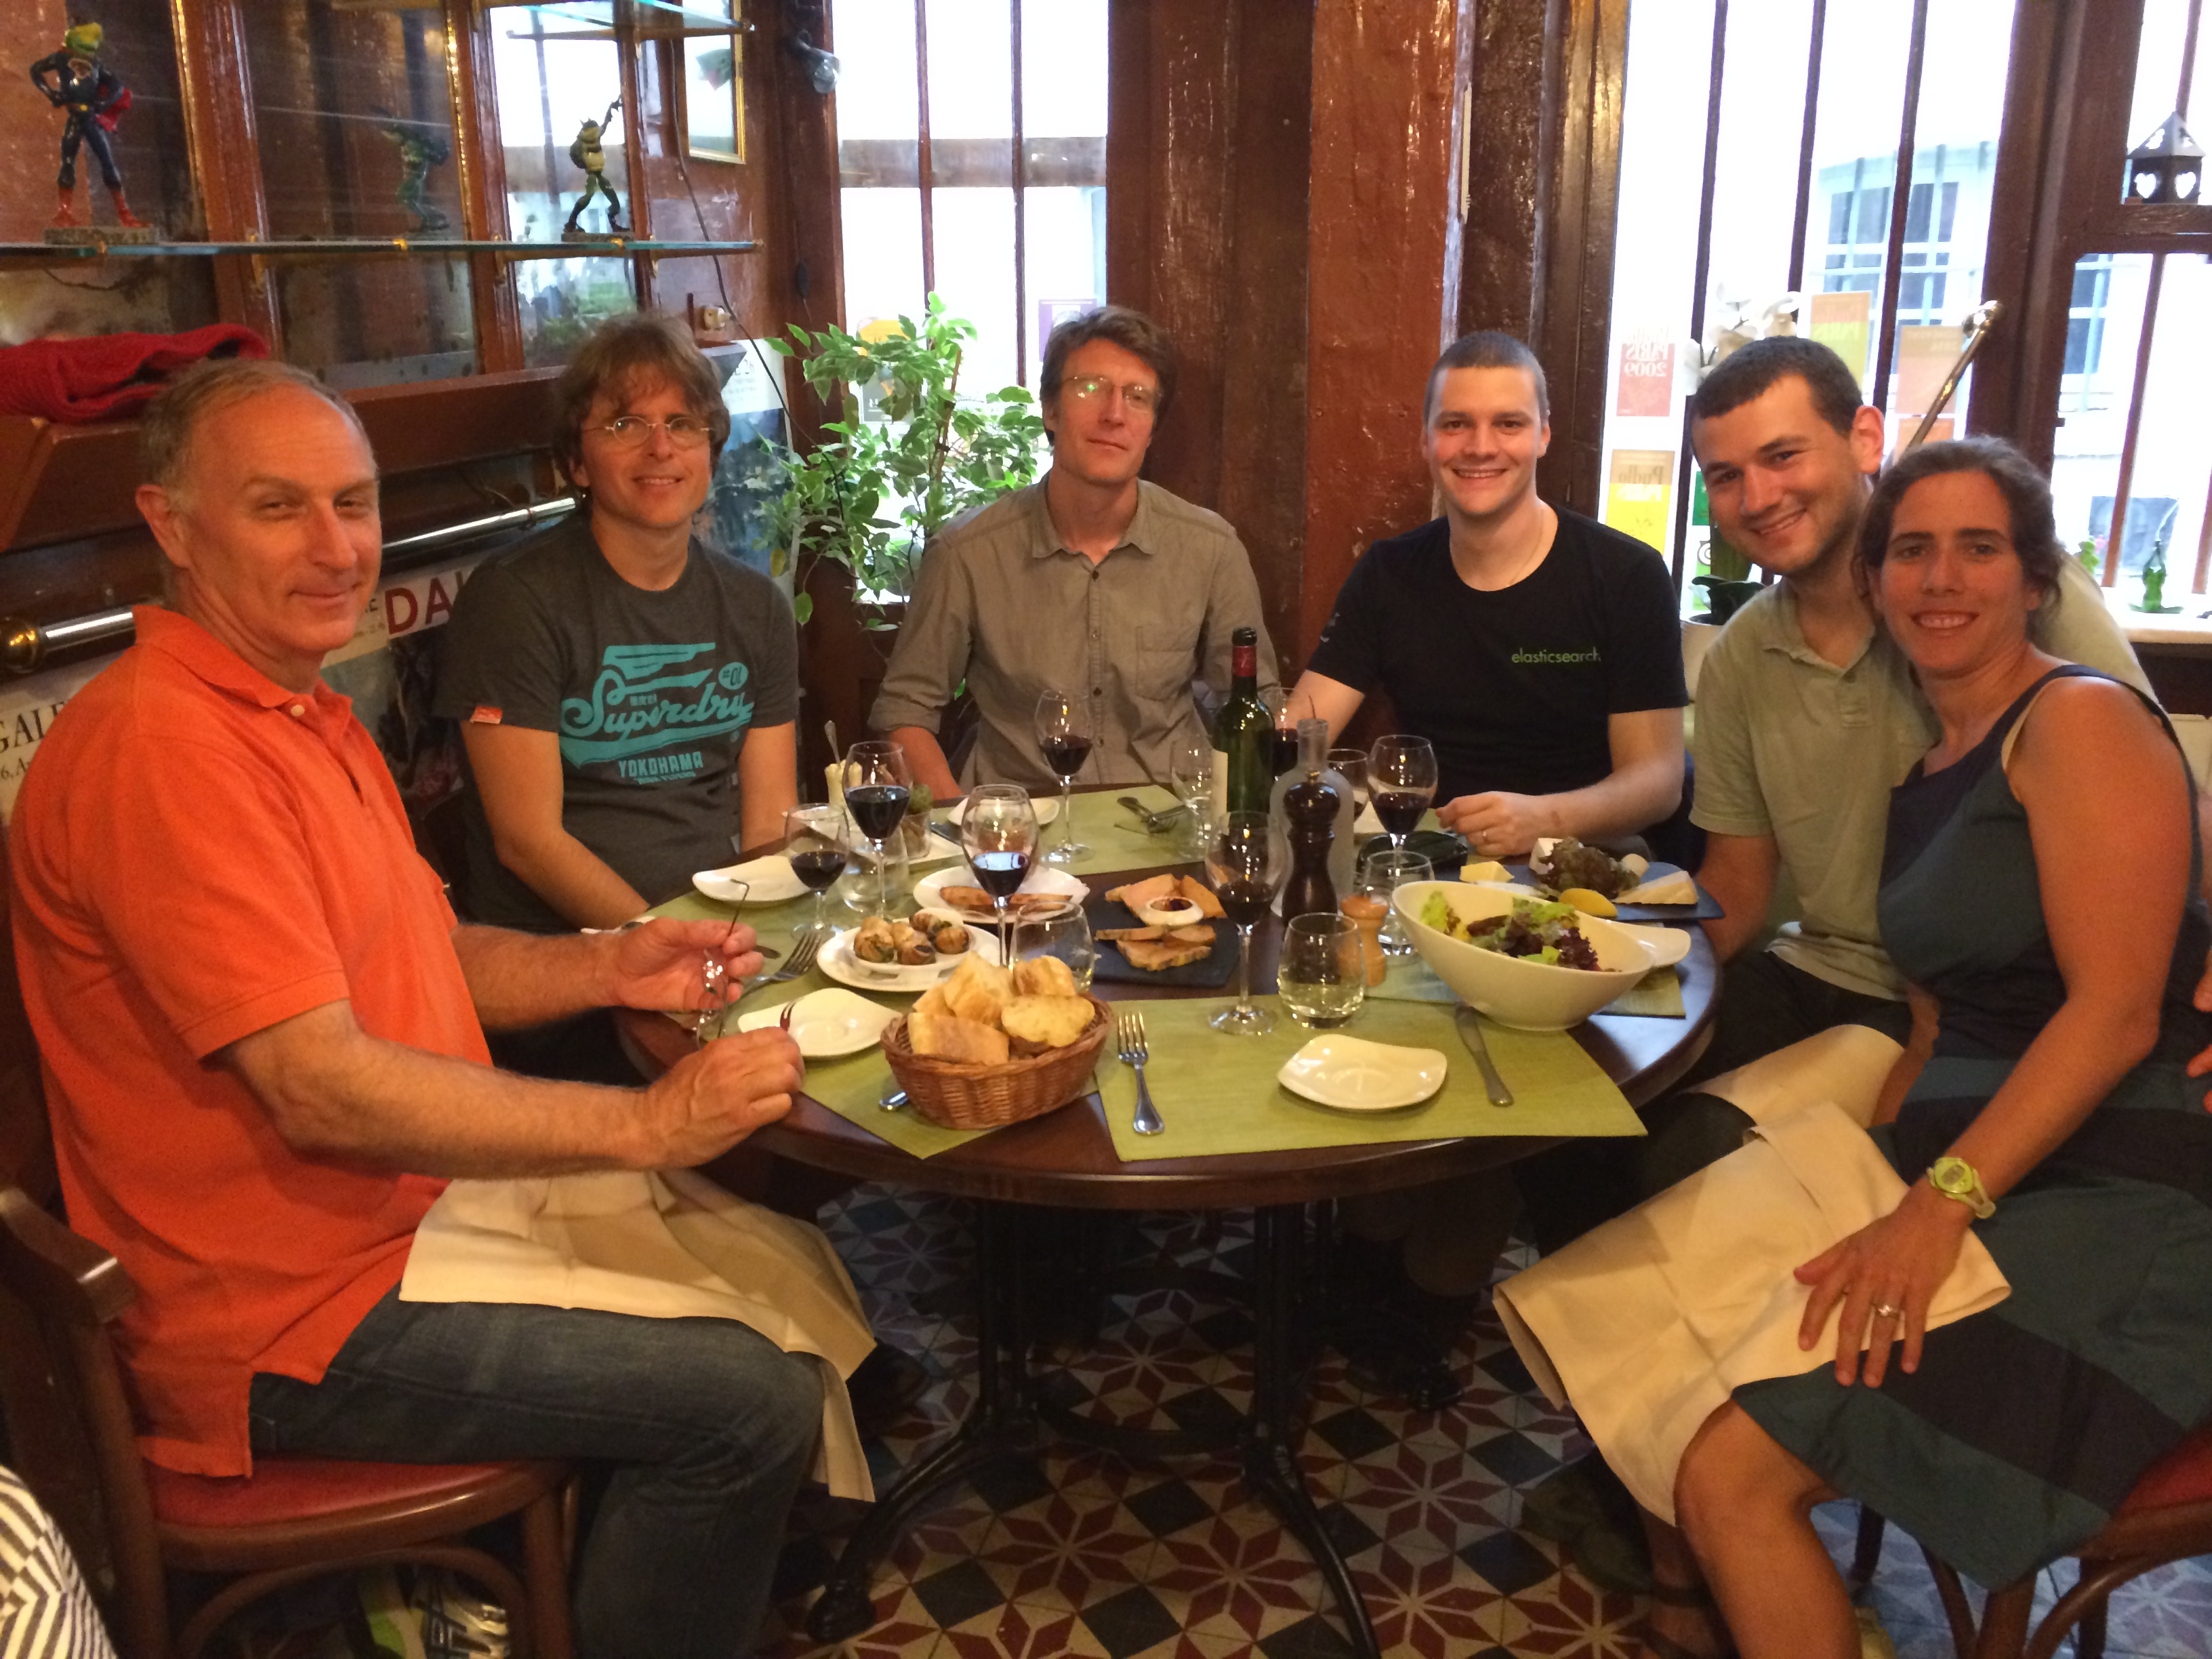
\includegraphics[width=3.5in]{dinner.jpg}
\end{center}
%\caption{The ``DSDN dinner''}
%\label{fig:Reinforcement}
%\end{figure}

\bibliographystyle{abbrv}
\bibliography{references}  % main.bib is the name of the Bibliography in this case

\end{document}
